\section{Internet und IP-Adressen}

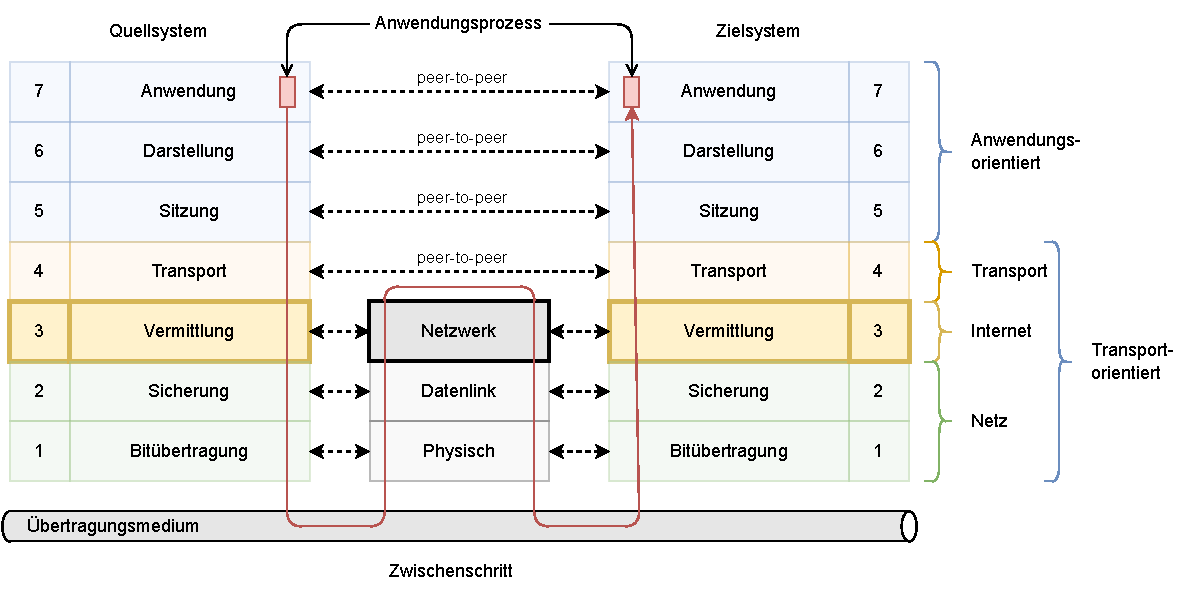
\includegraphics[width=\textwidth]{includes/figures/defi_iso_osi_network.pdf}

\subsection{Internet}

\begin{defi}{Internet}
    Das \emph{Internet}, ist ein weltweiter Verbund von Rechnernetzwerken, den autonomen Systemen.
    Router werden als koppelnde Elemente zwischen den Teilnetzen genutzt.
\end{defi}

\begin{bonus}{Aufbau des Internets}
    Die Basis des Internets bilden \emph{Tier 1} Internet Service Provider (ISPs).
    Diese treten gleichberechtigt untereinander auf und sind durch vertraglich regulierte Verbindungen angebunden.
    
    Als Verbindung zwischen den ISPs dienen \emph{Network Access Points} (NAPs) oder \emph{Internet Exchange Points} (IXPs)
    
    \begin{center}
        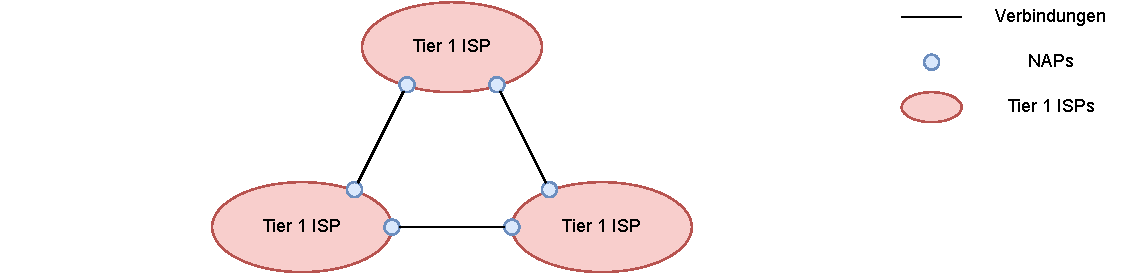
\includegraphics[width=0.75\textwidth]{includes/figures/bonus_aufbau_internet_1.pdf}
    \end{center}
    
    \emph{Tier 2} ISPs sind national bzw. regional und sind immer an einen oder mehrere Tier 1 ISPs angeschlossen.
    
    Sie treten dabei gegenüber \emph{Tier 1} ISPs als KundIn auf.
    
    \begin{center}
        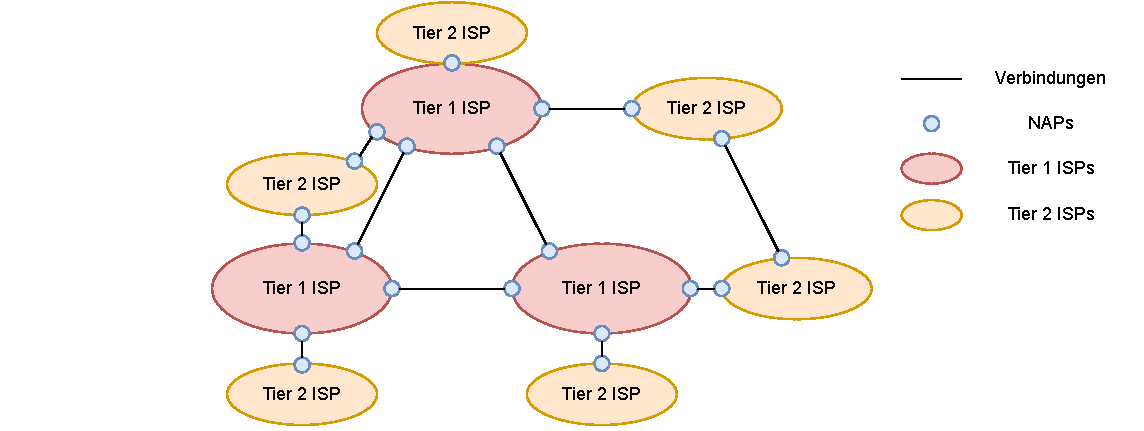
\includegraphics[width=0.75\textwidth]{includes/figures/bonus_aufbau_internet_2.pdf}
    \end{center}
    
    \emph{Tier 3} ISPs binden den bzw. die KundIn beispielsweise über DSL direkt an das gesamte Netzwerk an.
    
    Sie treten dabei gegenüber Tier 2 ISPs selber als KundIn auf.
    
    \begin{center}
        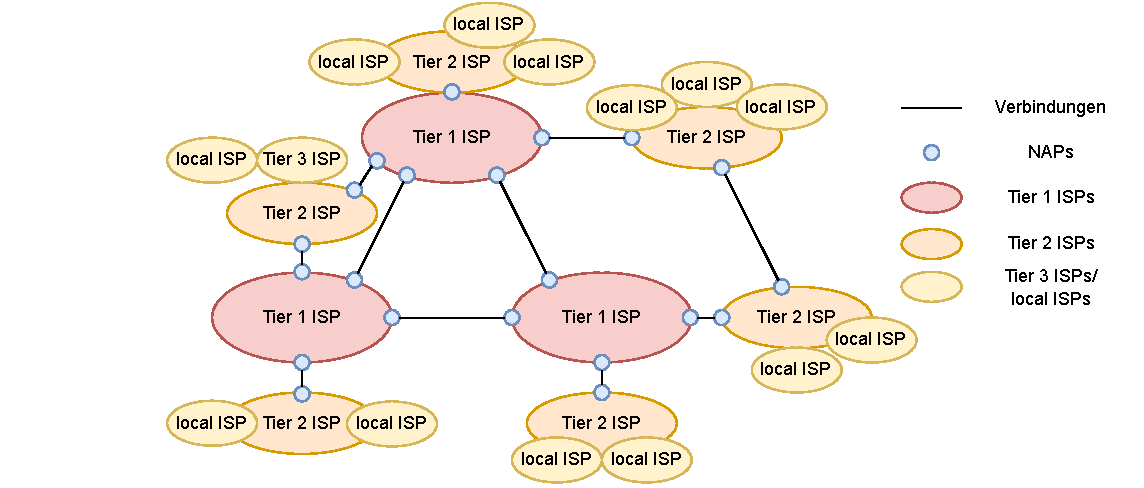
\includegraphics[width=0.75\textwidth]{includes/figures/bonus_aufbau_internet_3.pdf}
    \end{center}
\end{bonus}

\begin{bonus}{Aufbau des Internets}
    \begin{center}
        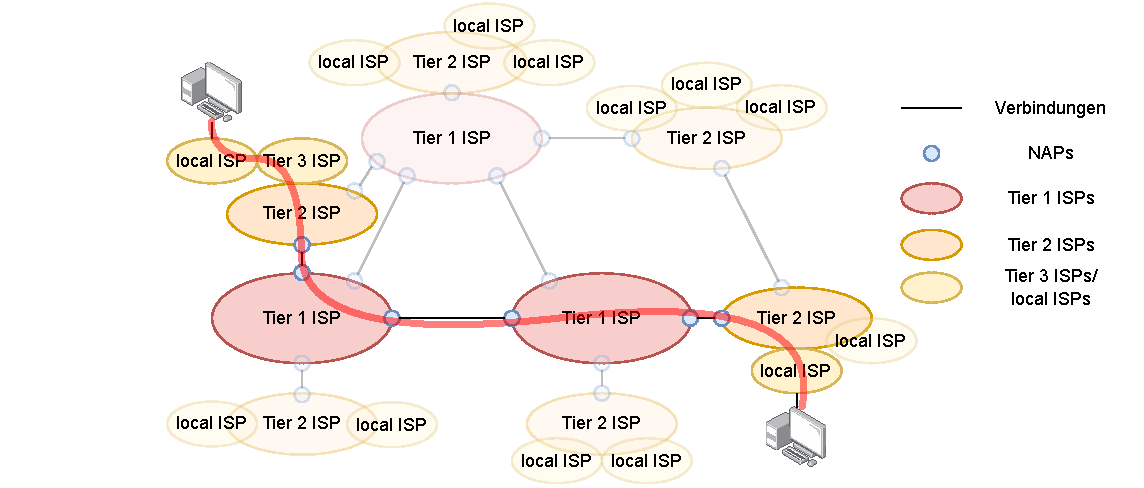
\includegraphics[width=0.75\textwidth]{includes/figures/bonus_aufbau_internet_4.pdf}
    \end{center}
\end{bonus}

\begin{bonus}{Nachrichtenzustellung}
    \begin{wrapfigure}{r}{0.25\textwidth}
        \begin{center}
            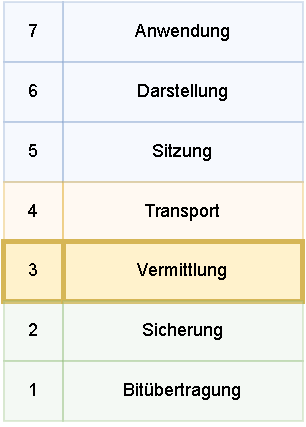
\includegraphics[width=0.2\textwidth]{includes/figures/bonus_iso_osi_vermittlung.pdf}
        \end{center}
    \end{wrapfigure}
    %
    Die Herausforderung in diesem großen Netz aus Netzen ist es Datenpakete von einem beliebigen Endgerät zu einem bestimmten Ziel zu versenden.
    
    Damit dies gelingt, wird in der Vermittlungsschicht einer der möglichen Wege zum Zielgerät gewählt.
    Die Wegwahl findet durch \emph{Routing-Protokolle} statt.
    
    Die Entscheidung erfolgt durch \emph{Routing-Tabellen}.
    In diesen lassen sich - je nach Protokoll - definierte Wege finden, unter denen man das autonome System des Zielgeräts findet bzw. welcher Weg befolgt werden soll, wenn das Zielgerät komplett unbekannt ist.
    
    In der Vermittlungsschicht wird größtenteils das IP-Protokoll genutzt, um die Pakete zu adressieren und Regeln zur Paketbehandlung aufzustellen.
\end{bonus}

\begin{defi}{Kapselung von Protokoll-Headern}
    Zur erfolgreichen Nachrichtenzustellung erweitern die verschiedenen Protokollinstanzen ein von einer Anwendung produziertes Datenpaket um verschiedene fest definierte Header.
    
    \begin{center}
        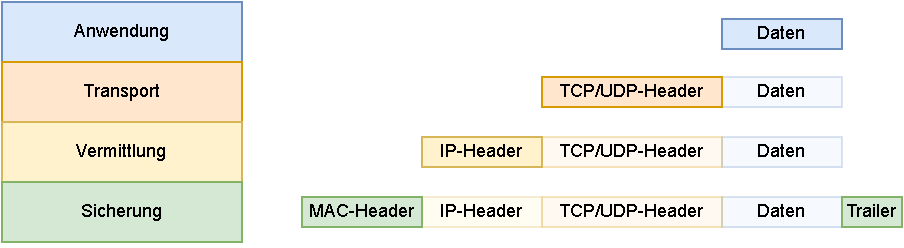
\includegraphics[width=0.75\textwidth]{includes/figures/defi_header_kapselung.pdf}
    \end{center}
    
    \begin{itemize}
        \item TCP bzw. UDP-Header dienen zur eindeutigen Prozessadressieren durch Ports.
        \item TCP sichert darüber hinaus die Datenübertragung
        \item IP-Header identifizieren ein eindeutiges Quell und Zielsystem
    \end{itemize}
    
    Demnach entsteht folgendes versandfertiges Datagramm:
    
    \begin{center}
        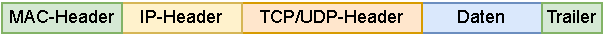
\includegraphics[width=0.75\textwidth]{includes/figures/defi_datagramm.pdf}
    \end{center}
\end{defi}

\subsection{IP}

\begin{defi}{Internet-Protokoll (IP)}
    Das \emph{Internet-Protokoll (IP)} bietet eine Ende-zu-Ende Kommunikation zwischen Endgeräten im Internet.
    Derzeit wird flächendeckend \emph{IPv4} bzw. \emph{IPv6} eingesetzt.
    
    IP ist paketvermittelnd, leitet also in sich geschlossene, unabhängige Dateneinheiten bzw. Datagramme ungesichert zwischen zwei Endpunkten weiter.
    Jedes Paket wird dabei in dem jeweiligen Router zwischengespeichert, überprüft und dementsprechend aussortiert oder weitergeleitet.
    
    Da die Pakete parallel von den Routern abgearbeitet werden, kann es passieren, dass:
    \begin{itemize}
        \item Datagramme verloren gehen
        \item Datagramme sich gegenseitig überholen
        \item Datagramme mehrfach ankommen
    \end{itemize}
    
    \emph{Sitzungen} werden durch einen exklusiven Kommunikationskanal über TCP simuliert.
\end{defi}

\begin{defi}{Wegwahl im Internet-Protokoll}
    Die IP-Implementierung eines Rechners oder Routers entscheidet eigenständig, wohin dieser ein Datagramm übertragen soll.
    
    Diese Entscheidung wird auf Basis von Routing- bzw. Forwarding-Tabellen getroffen.
    Dazu werden die Informationen, normalerweise ausschließlich die Zieladresse des Pakets, aus dem IP-Header in der jeweiligen Tabelle abgefragt.
    
    Router sind dabei meist an mehreren Netzen angeschlossen.
    Sie müssen zusätzlich noch überprüfen, ob sich das Zielgerät in einem anderen Netz befindet als das Quellgerät bzw. wie dieses Netz erreicht werden kann.
\end{defi}

\begin{example}{Wegwahl im Internet Protokoll}
    In folgendem Beispiel möchte \emph{Rechner A} an Paket an \emph{Rechner F} senden.
    
    \begin{center}
        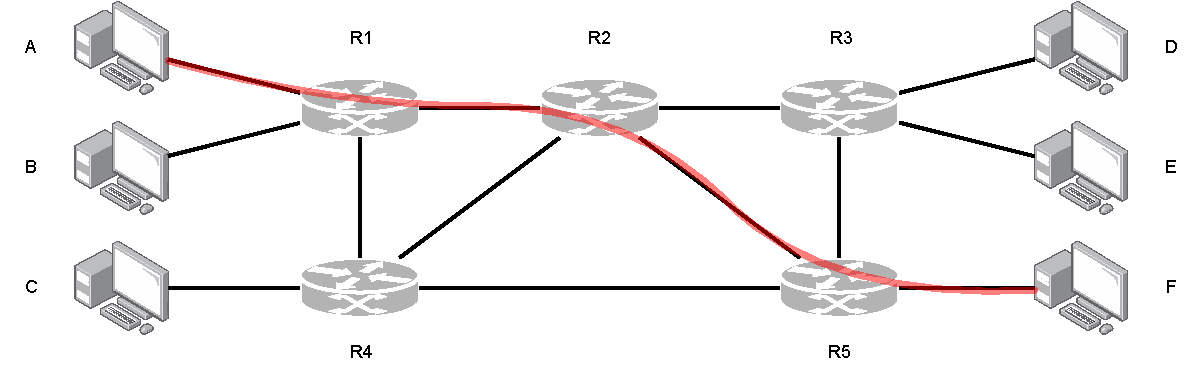
\includegraphics[width=0.75\textwidth]{includes/figures/example_ip_routing.pdf }
    \end{center}
    
    \begin{minipage}{0.25\textwidth}
        \begin{center}
            \emph{Rechner A}
            
            \begin{tabular}{|c|l|}
                \hline
                Ziel & Next Hop \\\hline\hline
                *    & $\to$ R1 \\\hline
            \end{tabular}
        \end{center}
    \end{minipage}
    \begin{minipage}{0.25\textwidth}
        \begin{center}
            \emph{R1}
            
            \begin{tabular}{|c|l|}
                \hline
                Ziel & Next Hop \\\hline\hline
                A    & A        \\
                B    & B        \\
                C    & R4       \\
                D    & R2       \\
                E    & R2       \\
                F    & $\to$ R2 \\\hline
            \end{tabular}
        \end{center}
    \end{minipage}
    \begin{minipage}{0.25\textwidth}
        \begin{center}
            \emph{R2}
            
            \begin{tabular}{|c|l|}
                \hline
                Ziel & Next Hop \\\hline\hline
                A    & R1       \\
                B    & R1       \\
                C    & R4       \\
                D    & R3       \\
                E    & R3       \\
                F    & $\to$ R5 \\\hline
            \end{tabular}
        \end{center}
    \end{minipage}
    \begin{minipage}{0.25\textwidth}
        \begin{center}
            \emph{R5}
            
            \begin{tabular}{|c|l|}
                \hline
                Ziel & Next Hop \\\hline\hline
                A    & R2       \\
                B    & R2       \\
                C    & R4       \\
                D    & R3       \\
                E    & R3       \\
                F    & $\to$ F  \\\hline
            \end{tabular}
        \end{center}
    \end{minipage}
\end{example}

\begin{defi}{IPv4-Adresse}
    Im Internet sind Endgeräte nicht über Namen erreichbar, sondern haben eine \emph{IP-Adresse}.
    
    Diese sind 32 bit bzw. 4 Byte lang und sind unterteilt in einen Bereich, um das Netz zu adressieren und einen Bereich um diesen Rechner in dem angegebenen Netz zu identifizieren.
    In Kombination ist die IP-Adresse (theoretisch) weltweit eindeutig.
    
    Zur einfachen und übersichtlichen Darstellung werden IP-Adressen in vier Blöcke mit je einem Byte aufgeteilt, von denen jeder eine dezimale Zahl darstellt.
    
    Ein Beispiel ist das Klasse B Netz der RWTH Aachen University \texttt{134.130.0.0}.
\end{defi}

\begin{defi}{IPv4-Adressklassen}
    Um die verfügbaren IP-Adressen fair und sinnvoll aufzuteilen, wurden \emph{Klassen} definiert.
    Mithilfe dieser Klassen können Anfragen von KundInnen, je nach benötigter Anzahl von IP-Adressen, schnell bearbeitet werden.
    
    \begin{enumerate}[label=Klasse \Alph*:, leftmargin=*]
        \item Für Netze mit bis zu 16 Mio. Knoten
              
              (Knoten-ID: $0\text{-}127$, 50\% des IPv4-Adressraums)
    \end{enumerate}
    
    \begin{center}
        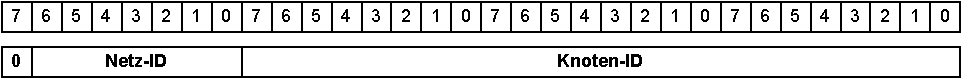
\includegraphics[width=0.75\textwidth]{includes/figures/bonus_class_a.pdf}
    \end{center}
    
    \begin{enumerate}[label=Klasse \Alph*:, leftmargin=*, start=2]
        \item Für Netze mit bis zu 65.536 Knoten
              
              (Knoten-ID: $128\text{-}191$, 25\% des IPv4-Adressraums)
    \end{enumerate}
    
    \begin{center}
        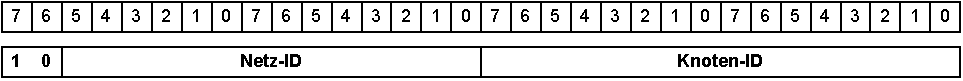
\includegraphics[width=0.75\textwidth]{includes/figures/bonus_class_b.pdf}
    \end{center}
    
    \begin{enumerate}[label=Klasse \Alph*:, leftmargin=*, start=3]
        \item Für Netze mit bis zu 256 Knoten
              
              (Knoten-ID: $192\text{-}223$, 12.5\% des IPv4-Adressraums)
    \end{enumerate}
    
    \begin{center}
        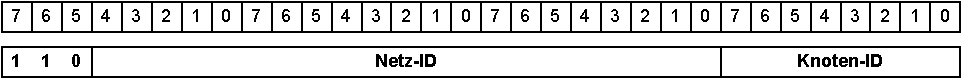
\includegraphics[width=0.75\textwidth]{includes/figures/bonus_class_c.pdf}
    \end{center}
    
    \begin{enumerate}[label=Klasse \Alph*:, leftmargin=*, start=4]
        \item Für Gruppenkommunikation
              
              (Knoten-ID: $224\text{-}239$, 6.25\% des IPv4-Adressraums)
    \end{enumerate}
    
    \begin{center}
        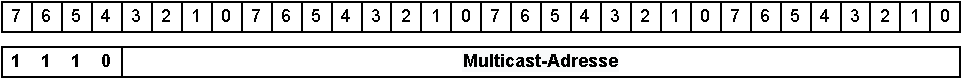
\includegraphics[width=0.75\textwidth]{includes/figures/bonus_class_d.pdf}
    \end{center}
    
    \begin{enumerate}[label=Klasse \Alph*:, leftmargin=*, start=5]
        \item Reserviert für zukünftige Anwendungen
              
              (Knoten-ID: $240\text{-}255$, 6.25\% des IPv4-Adressraums)
    \end{enumerate}
    
    \begin{center}
        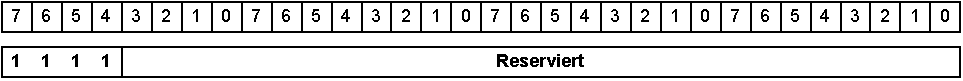
\includegraphics[width=0.75\textwidth]{includes/figures/bonus_class_e.pdf}
    \end{center}
    
    In allen Netzen ist die Knoten-ID \texttt{0..0} ($0$) für das Netz selber reserviert.
    
    Des Weiteren wird für Broadcast Nachrichten an alle teilnehmenden Geräte im Netz die Knoten-ID \texttt{1..1} (A: 127, B: 191, bzw. C: 223) genutzt.
\end{defi}

\begin{bonus}{Loopback-Adresse}
    Um Kommunikation mit Anwendungen auf dem selben Rechner zu führen, kann man die IPv4-Adresse \texttt{127.0.0.1} nutzen.
    Diese virtuelle Netzwerkkarte verfolgt nicht die tieferen Schichten des ISO-OSI-Modells, sondern geht \enquote{zurück} über die Transportschicht an die angesprochene Anwendung.
\end{bonus}

\begin{defi}{IP-Subnetze}
    Wenn wir nun die bestehenden Netzwerkklassen mit unseren neuen bekannten Subnetzmasken zusammenfügen, können wir große Netze in kleine durch Router getrennte Bereiche aufteilen.
    
    Aufgrund des Präfix erkennt man an der IPv4-Adresse die Adressklasse.
    Anhand der Subnetzmaske erkennt man die Länge der Netz-ID.
    
    Stimmen die Längen der Netz-ID der Adressklasse und die Gesamtlänge der Netz-ID überein, haben wir keine Subnetze.
    Ist die Gesamtlänge der Netz-ID länger, können wir errechnen, wie viele Subnetze möglich sind.
\end{defi}

\begin{defi}{IP-Header}
    \begin{center}
        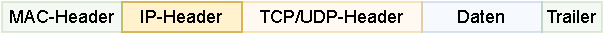
\includegraphics[width=0.75\textwidth]{includes/figures/defi_ip_header_kapselung.pdf}
        
        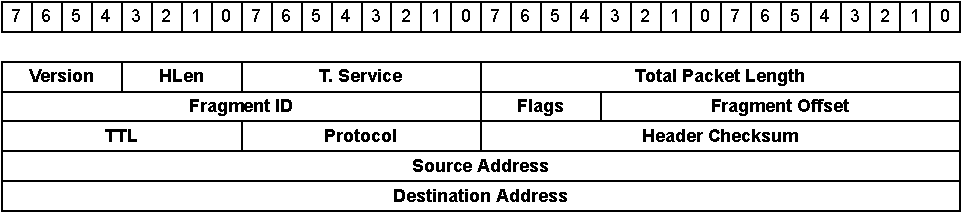
\includegraphics[width=0.75\textwidth]{includes/figures/defi_ip_header.pdf}
    \end{center}
\end{defi}